\documentclass[a4paper,11pt]{article}
\usepackage{amsmath,amsthm,amsfonts,amssymb,amscd,amstext,vmargin,graphics,graphicx,tabularx,multicol} \usepackage[french]{babel}
\usepackage[utf8]{inputenc}  
\usepackage[T1]{fontenc} 
\usepackage[T1]{fontenc}
\usepackage{amsmath,amssymb}
\usepackage{pstricks-add,tikz,tkz-tab,variations}
\usepackage[autolanguage,np]{numprint} 
\usepackage{color}
\usepackage{ulem}

\setmarginsrb{1.5cm}{0.5cm}{1cm}{0.5cm}{0cm}{0cm}{0cm}{0cm} %Gauche, haut, droite, haut
\newcounter{numexo}
\newcommand{\exo}[1]{\stepcounter{numexo}\noindent{\bf Exercice~\thenumexo} : \marginpar{\hfill /#1}}
\reversemarginpar


\newcounter{enumtabi}
\newcounter{enumtaba}
\newcommand{\q}{\stepcounter{enumtabi} \theenumtabi)  }
\newcommand{\qa}{\stepcounter{enumtaba} (\alph{enumtaba}) }
\newcommand{\initq}{\setcounter{enumtabi}{0}}
\newcommand{\initqa}{\setcounter{enumtaba}{0}}

\newcommand{\be}{\begin{enumerate}}
\newcommand{\ee}{\end{enumerate}}
\newcommand{\bi}{\begin{itemize}}
\newcommand{\ei}{\end{itemize}}
\newcommand{\bp}{\begin{pspicture*}}
\newcommand{\ep}{\end{pspicture*}}
\newcommand{\bt}{\begin{tabular}}
\newcommand{\et}{\end{tabular}}
\renewcommand{\tabularxcolumn}[1]{>{\centering}m{#1}} %(colonne m{} centrée, au lieu de p par défault) 
\newcommand{\tnl}{\tabularnewline}

\newcommand{\trait}{\noindent \rule{\linewidth}{0.2mm}}
\newcommand{\hs}[1]{\hspace{#1}}
\newcommand{\vs}[1]{\vspace{#1}}

\newcommand{\N}{\mathbb{N}}
\newcommand{\Z}{\mathbb{Z}}
\newcommand{\R}{\mathbb{R}}
\newcommand{\C}{\mathbb{C}}
\newcommand{\Dcal}{\mathcal{D}}
\newcommand{\Ccal}{\mathcal{C}}
\newcommand{\mc}{\mathcal}

\newcommand{\vect}[1]{\overrightarrow{#1}}
\newcommand{\ds}{\displaystyle}
\newcommand{\eq}{\quad \Leftrightarrow \quad}
\newcommand{\vecti}{\vec{\imath}}
\newcommand{\vectj}{\vec{\jmath}}
\newcommand{\Oij}{(O;\vec{\imath}, \vec{\jmath})}
\newcommand{\OIJ}{(O;I,J)}

\newcommand{\bmul}[1]{\begin{multicols}{#1}}
\newcommand{\emul}{\end{multicols}}


\newcommand{\reponse}[1][1]{%
\multido{}{#1}{\makebox[\linewidth]{\rule[0pt]{0pt}{20pt}\dotfill}
}}

\newcommand{\titre}[5] 
% #1: titre #2: haut gauche #3: bas gauche #4: haut droite #5: bas droite
{
\noindent #2 \hfill #4 \\
#3 \hfill #5

\vspace{-1.6cm}

\begin{center}\rule{6cm}{0.5mm}\end{center}
\vspace{0.2cm}
\begin{center}{\large{\textbf{#1}}}\end{center}
\begin{center}\rule{6cm}{0.5mm}\end{center}
}



\begin{document}
\pagestyle{empty}
\titre{Contrôle 1 : Théorème de Pythagore, de Thalès et les statistiques }{Nom}{Prénom}{Date}{Classe}

\begin{flushleft}
\begin{tabular}{|m{9.5cm}|m{1.25cm}|m{1.25cm}|m{1.25cm}|m{1.25cm}|m{1.25cm}|}
\hline 
\textbf{Compétences} & \begin{center}
\textbf{N.E.}
\end{center} & \begin{center}
\textbf{M.I.}
\end{center} & \begin{center}
\textbf{M.F.}
\end{center}  & \begin{center}
\textbf{M.S.}
\end{center} & \begin{center}
\textbf{T.B.M.}
\end{center} \\ 
\hline 
Je dois savoir traduire en langage mathématique une situation réelle &  &  & & &\\
\hline 
Je dois savoir extraire d'un document les informations utiles, les reformuler, les organiser, les confronter à mes connaissances &  &  & & &\\
\hline
\end{tabular} 
\end{flushleft}

\textit{N.E = Non évalué ; M.I. = Maîtrise insuffisante ; M.F. = Maîtrise fragile ; M.S. = Maîtrise satisfaisante ; T.B.M. = Très bonne maîtrise}\\


\vspace*{0.25cm}

\exo{5} \\
Cet exercice est un questionnaire à choix multiples.\\
Pour chaque question, quatre réponses sont proposées mais une seule est exacte. Pour chacune des questions, entourer la bonne réponse, aucune justification n'est demandée.\\

\vspace*{0.25cm}

\renewcommand{\arraystretch}
{3.2}

\begin{tabular}{|c|p{9cm}|p{2.5cm}|p{2.35cm}|p{2.35cm}|}
\hline 
 & \textbf{Questions} & \textbf{Réponse B} & \textbf{Réponse B} & \textbf{Réponse C} \\ 
\hline 
\textbf{1} & L'écriture décimale du nombre $15,3 \times 10^{5}$ est : & 1 530 000 & 15,300000 & 15 300 000 \\ 
\hline 
\textbf{2} & La notation scientifique de 1 500 000 000 est : & $15 \times 10^{-8}$ & $15 \times 10^{8}$ & $1,5 \times 10^{9}$ \\
\hline 
\textbf{3} & $\dfrac{5}{3}-\dfrac{1}{3} \times \dfrac{3}{2}$ est égal à : & $\dfrac{2}{3}$ & $\dfrac{7}{6}$  & 2 \\ 
\hline 
\textbf{4} & Une solution de l'équation $ 2x+3=7x-4$ est : & $\dfrac{5}{7}$ & 1,4 & -0,7 \\ 
\hline 
\textbf{5 }& On donne le triangle suivant :
\includegraphics[scale=0.85]{qcmreciproque.eps}  & Le triangle ABC est rectangle en C & Le triangle ABC n'est pas rectangle & On ne peut pas savoir \\ 
\hline 
\end{tabular} 

\vspace*{1cm}


\exo{4} Cindy, Eric et Kevin se sont partagés 89  cartes Pokemon. \\
Cindy a pris trois fois plus de carte que Eric et Kevin a pris 5 carte de plus
que Cindy.\\
 Combien ont-ils de cartes Pokemon chacun ? \textit{(Résoudre le problème à l'aide d'une équation)}

\newpage

\exo{3} Thomas attache son cerf-volant au sol au point T.\\
Il fait 20 pas pour parcourir la distance TH.
Un pas mesure 0,6 mètre.\\
Le schéma ci-dessous illustre la situation. Il n'est pas à l'échelle.\\
\textbf{Montrer que la hauteur CH du cerf-volant est
égale à 9 m.}

\begin{center}
\includegraphics[scale=0.8]{controle1.eps} 
\end{center}



\vspace*{0.5cm}

\exo{4} Un professeur de SVT demande aux 29 élèves d'une classe de sixième de faire germer des graines de blé chez eux.

Le professeur donne un protocole expérimental à suivre.
\bi
\item Mettre en culture sur du coton dans une boîte placée dans une pièce éclairée, de température entre \\
20 \degre C et 25\degre C.
\item Arroser une fois par jour.
\item Il est possible de couvrir les graines avec un film transparent pour éviter l'évaporation de l'eau.\\
\ei

Le tableau ci-dessous donne les tailles des plantules (petites plantes) des 29 élèves à 10 jours après la mise en germination.\\


\renewcommand{\arraystretch}{1.8}

\begin{tabular}{|c|c|c|c|c|c|c|c|c|c|c|c|}
\hline 
\textbf{Taille (en cm)} & 0 & 8 & 12 & 14 & 16 & 17 & 18 & 19 & 20 & 21 & 22 \\ 
\hline 
\textbf{Effectifs} & 1 & 2 & 2 & 4 & 2 & 2 & 3 & 3 & 4 & 4 & 2 \\ 
\hline 
\end{tabular} 

\vspace*{0.4cm}

\initq \q Donner les valeurs extrêmes de cette série.\\



\q On considère qu'un élève a bien respecté le protocole si la taille de la plantule à 10 jours est supérieure ou égale à 14 cm.\\
Quel pourcentage des élèves de la classe a bien respecté le protocole ?\\

\q Calculer la moyenne de cette série et interpréter votre résultat. Arrondir au dixième près.\\


\exo{4}\\

M. Dupond et M. Durand ont chacun une entreprise de 100 personnes. Nous avons les informations suivantes :\\

\begin{tabular}{|c|c|c|}
\hline 
\textbf{Âge moyen} & M. Dupond & M. Durand \\ 
\hline 
\textbf{Hommes}  & 51 & 54 \\ 
\hline 
\textbf{Femmes} & 36 & 39 \\ 
\hline 
\end{tabular} \hspace*{2.25cm} \begin{tabular}{|c|c|c|}
\hline 
\textbf{Effectif} & M. Dupond & M. Durand \\ 
\hline 
\textbf{Hommes}  & 50 & 20 \\ 
\hline 
\textbf{Femmes} & 50 & 80 \\ 
\hline 
\end{tabular} \\

\vspace*{0.5cm}

\initq \q A l'aide des tableaux ci-dessus, décrire en 2 phrases la composition de l'entreprise de M. Durand et celle de M. Dupond.\\

\q Hugo dit à son frère : " En moyenne, les personnes de l'entreprise de M. Durand sont plus vieille que celles de l'entreprise de M. Dupond."\\
Qu'en pensez-vous ?\\

\textit{Toute trace de recherche, même incomplète, ou d'initiative même infructueuse, sera prise en compte dans l'évaluation.}


\end{document}
